% !TeX spellcheck = en_US
\section{Problem 10}

\subsection{Question A}

The patterns that we want to separate are plotted in figure~\ref{fig:prob_10_patterns}.

\begin{figure}[htpb]
	\centering
	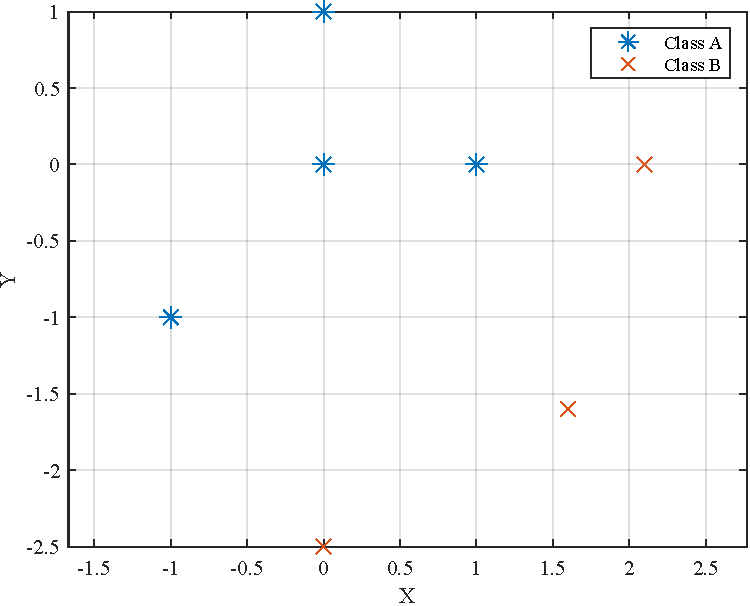
\includegraphics[width=0.5\textwidth]{../Problem 10/patterns.pdf}
	\caption{Plot of patterns}
	\label{fig:prob_10_patterns}
\end{figure}

We can clearly see that there is a straight line that can separate the two classes, thus an ADALINE neural network can work in classification for this system.